\documentclass[ignorenonframetext,10pt,aspectratio=169]{beamer}

\usepackage{umut}
\usepackage{umuttr}
\usepackage{usynsem}
\usepackage[utf8]{inputenc}
\usepackage{uling}
\usepackage{natbib,unatbib}
\usepackage{linguex}
         \renewcommand{\refdash}{}
\usepackage{ubeamer}
\usepackage{verbatim}
\usepackage{adjustbox}
\usepackage{fancyvrb}

\usepackage{tikz-qtree}
\usetikzlibrary{er,positioning}

\title{Functional Projections}
\author{\  \\  {\it Partly based on Koeneman \& Zeiljstra (2017)} \\ \vspace{20pt} Umut \"Ozge\\  }

\date{COGS 532: Theoretical Linguistics\\ METU, Informatics}

\begin{document}

\begin{frame}\frametitle{}
\thispagestyle{empty}
\maketitle
\end{frame}

\begin{frame}[t,plain]{Lexical versus functional projections}

		\begin{center}
				\vspace{60pt}\hspace{80pt}
\adjustbox{valign=t}{
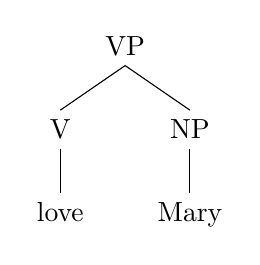
\begin{tikzpicture}
\tikzset{level distance=30pt, sibling distance=20pt}
				\Tree
					[.{VP}
					[.{V} love ] 
					[.{NP} Mary ] 
					]
\end{tikzpicture}}
		\end{center}
\end{frame}

\begin{frame}[t,plain]{Lexical versus functional projections}

\begin{center}
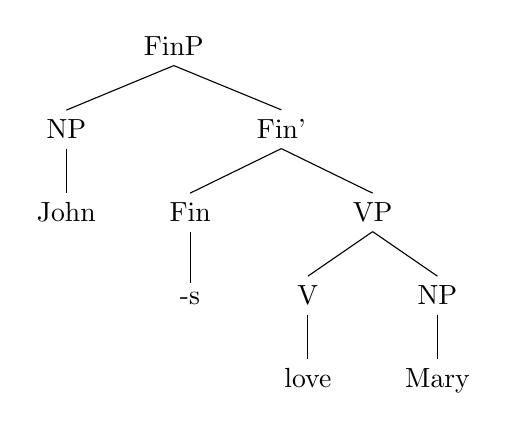
\begin{tikzpicture}
\tikzset{level distance=30pt, sibling distance=20pt}
				\Tree
				[.{FinP}
					[.{NP} John ]
					[.{Fin'} 
						[.{Fin} -s ]
							[.{VP}
								[.{V} love ] 
								[.{NP} Mary ] 
							]
					]
				]
\end{tikzpicture}
\end{center}

\end{frame}

\begin{frame}[t,plain]{Determiner Phrases}
\ex. \paradigm{\text{this}\\ \text{that}\\ \text{the}\\ \text{a}\\ \text{no}\\ \text{her}\\ \text{John's}\\ \text{the woman's}} panic

\end{frame}

\begin{frame}[t,plain]{Determiner Phrases}

\begin{center}
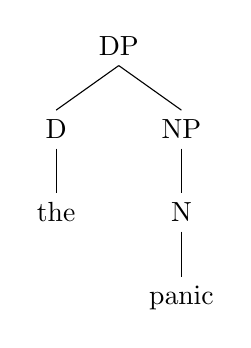
\begin{tikzpicture}
\tikzset{level distance=30pt, sibling distance=20pt}
				\Tree
				[.{DP} 
					[.{D} the ]
					[.{NP} [.{N} panic ] ]
				]
\end{tikzpicture}
\end{center}
\end{frame}

\begin{frame}[t,plain]{Determiner Phrases}

\begin{center}
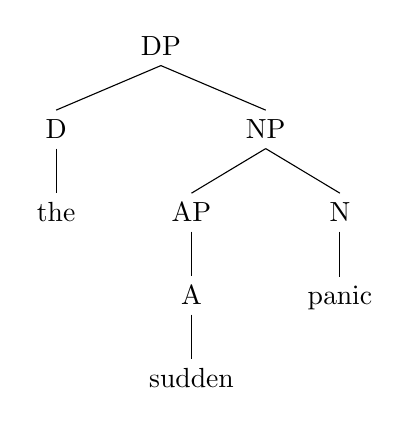
\begin{tikzpicture}
\tikzset{level distance=30pt, sibling distance=20pt}
				\Tree
				[.{DP} 
					[.{D} the ]
					[.{NP}
 						[.{AP}
							[.{A} sudden ]
						]
						[.{N} panic ]
					]
				]
\end{tikzpicture}
\end{center}
\end{frame}

\begin{frame}[t,plain]{Determiner Phrases}

\begin{center}
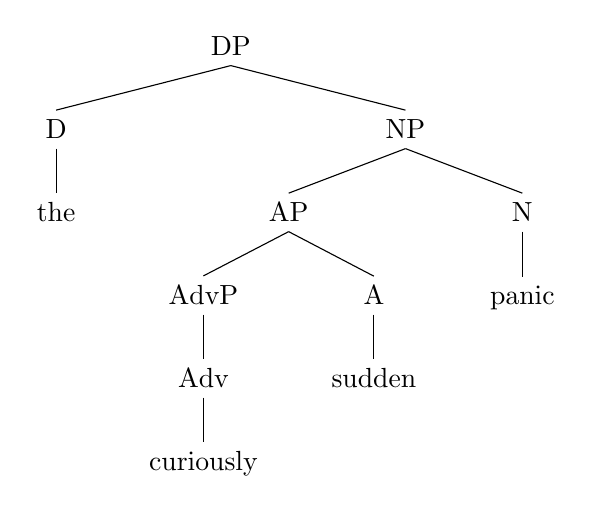
\begin{tikzpicture}
\tikzset{level distance=30pt, sibling distance=20pt}
				\Tree
				[.{DP} 
					[.{D} the ]
					[.{NP}
 						[.{AP}
							[.{AdvP} 
								[.{Adv} curiously ]
							]
							[.{A} sudden ]
						]
						[.{N} panic ]
					]
				]
\end{tikzpicture}
\end{center}
\end{frame}

\begin{frame}[t,plain]{Determiner Phrases}

\begin{center}
\begin{tikzpicture}
\tikzset{level distance=30pt, sibling distance=20pt}
				\Tree
				[.{DP} 
					[.{D} the ]
					[.{NP}
 						[.{AP}
							[.{AdvP} 
								[.{Adv} curiously ]
							]
							[.{A} sudden ]
						]
						[.{N'}
							[.{N} panic ]
							[.{PP}
								[.{P} in ]
								[.{DP}
									[.{D} the ]
									[.{NP} \edge[roof]; woods ]
								]
							]
						]
					]
				]
\end{tikzpicture}
\end{center}
\end{frame}

\begin{frame}[t,plain]{The Possessive}

		\ex. The neighbor's car.

\begin{center}
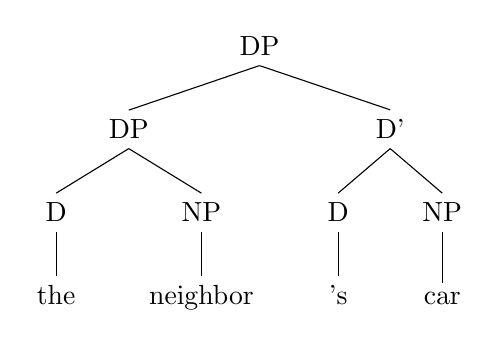
\begin{tikzpicture}
\tikzset{level distance=30pt, sibling distance=20pt}
				\Tree
				[.{DP}
					[.{DP} 
						[.{D} the ]
						[.{NP} neighbor ]
						]
					[.{D'} 
						[.{D} 's ]
						[.{NP} car ]
					]
				]
\end{tikzpicture}
\end{center}
\end{frame}

\begin{frame}[t,plain]{Some parallels}

\adjustbox{valign=t}{
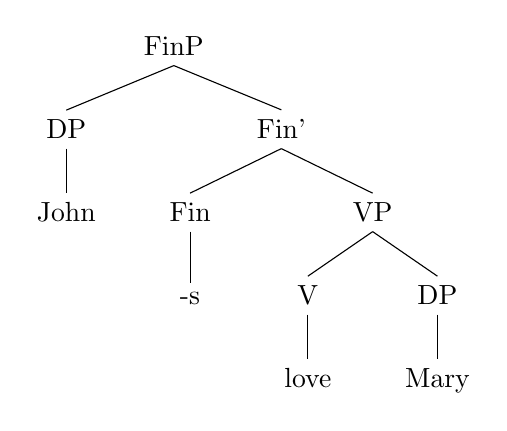
\begin{tikzpicture}
\tikzset{level distance=30pt, sibling distance=20pt}
				\Tree
				[.{FinP}
					[.{\alert{DP}} John ]
					[.{Fin'} 
						[.{Fin} -s ]
							[.{VP}
								[.{V} love ] 
								[.{\alert{DP}} Mary ] 
							]
					]
				]
\end{tikzpicture}}
\hspace{50pt}
\adjustbox{valign=t}{
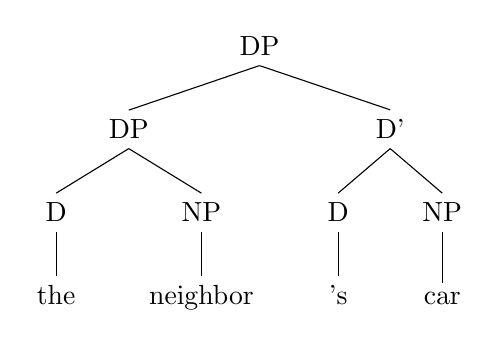
\begin{tikzpicture}
\tikzset{level distance=30pt, sibling distance=20pt}
				\Tree
				[.{DP}
					[.{DP} 
						[.{D} the ]
						[.{NP} neighbor ]
						]
					[.{D'} 
						[.{D} 's ]
						[.{NP} car ]
					]
				]
\end{tikzpicture}}

\end{frame}

\begin{frame}[t,plain]{Terminology on functional projections}

		\vspace{30pt}
		\begin{center}
\adjustbox{valign=t}{
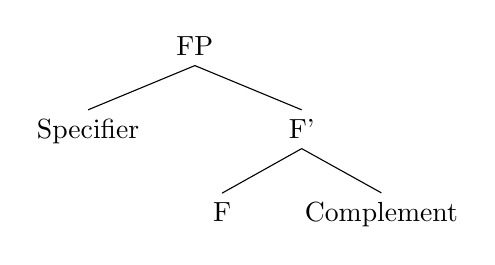
\begin{tikzpicture}
\tikzset{level distance=30pt, sibling distance=20pt}
				\Tree
				[.{FP}
					[.{Specifier} ]
					[.{F'} 
						[.{F} ]
						[.{Complement} ]
					]
				]
\end{tikzpicture}}

		\end{center}

\end{frame}

\begin{frame}[t,plain]{Complement Phrases}

\ex. John believes that Mary is a genius.

\begin{center}
\adjustbox{valign=t}{
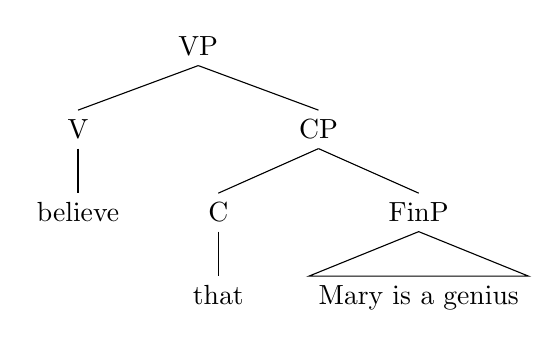
\begin{tikzpicture}
\tikzset{level distance=30pt, sibling distance=20pt}
				\Tree
				[.{VP}
					[.{V} believe ]
					[.{CP} 
						[.{C} that ]
						[.{FinP} \edge[roof]; {Mary is a genius} ]
					]
				]
\end{tikzpicture}}
\end{center}



\end{frame}

\begin{frame}[t,plain]{}

\end{frame}

\begin{frame}[t,plain]{}

\end{frame}

\begin{frame}[t,plain]{}

\end{frame}

\begin{frame}[t,plain]{}

\end{frame}

\begin{frame}[t,plain]{}

\end{frame}

\begin{frame}[t,plain]{}

\end{frame}

\end{document}
